% Two sources of nonconvexity, each giving several local minima.
%
%   figures/tikz/ci-contours-nonconvex.tex
%       -> media/figures/ci-contours-nonconvex.{png,svg}
%
% Lecture 18 (Introduction to Constrained Optimization), "A taxonomy of contour plots".
% Drawn 2026-10-07 for the two pictures Biegler shows as Fig. 4.3 (p. 67), which the lecture
% had only described in words, with the 2018 notes' captions "nonconvex region with multiple
% optima" and "nonconvex objective" (3 local optima). Our own geometry.
%
% PANEL (1): convex objective, nonconvex region.
%   F = annular sector {1 <= r <= 1.6, 30 deg <= theta <= 150 deg} (an arch; the chord
%   between its two feet leaves it). f = |x - c|^2 with c = (0.2,-0.5), marked "+".
%   On the inner arc, |u(theta) - c|^2 = 1.29 - 0.4 cos(theta) + sin(theta), whose only
%   stationary point in (30,150) deg is a maximum (tan theta = -2.5, theta = 111.8 deg), so
%   the arc's minima are its two ends. At each end both feasible directions (along the arc,
%   radially outward) have positive directional derivative, so both are STRICT LOCAL MINIMA:
%     (0.866, 0.5): f = 1.4436 (distance 1.2015), the global minimizer;
%     (-0.866,0.5): f = 2.1364 (distance 1.4616), local only.
%   No other local minima: f increases outward along every radius (u.c <= -0.077 < 1), and the
%   outer arc is at distance >= 1.76. Contours: circles of radius 0.6 (dashed), 1.2015 and
%   1.4616 (solid; each touches F at one foot), 1.9 (dashed).
%
% PANEL (2): convex region, nonconvex objective.
%   F = pentagon (0,0), (3,0), (3,1.6), (1.6,2.5), (0,1.9).
%   f(x) = 0.15 |x - (1.5,1.1)|^2 - 1.0 exp(-|x - (0.6,0.6)|^2/0.15)
%          - 0.75 exp(-|x - (2.3,0.8)|^2/0.15) - 0.9 exp(-|x - (1.4,1.8)|^2/0.15).
%   Local minima over F, found on a 0.01 grid restricted to F and refined with scipy BFGS:
%     (0.620,0.611) f = -0.8445 (global); (1.402,1.783) f = -0.8268; (2.277,0.809) f = -0.6437.
%   Exactly three, all interior, none on the boundary. Contours f = -0.7, -0.5, -0.25, 0.05
%   from matplotlib's contour on that grid, every 6th point (every 3rd for short loops). At
%   f = -0.7 only two wells have a loop, since the third well bottoms out at -0.6437.
%
% Neither panel marks the local minima: the lecture's activity asks students to find them.
%
% GREYSCALE: F is hatched in both panels; contours are grey; "+" marks the unconstrained
% minimizer of f in panel (1). Nothing is carried by colour alone.
\usetikzlibrary{patterns}
\definecolor{okabeblue}{HTML}{0072B2}

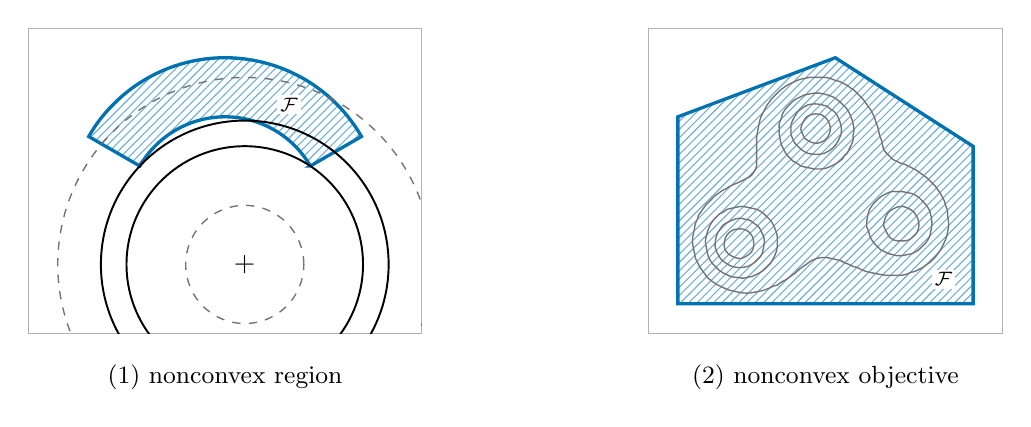
\begin{tikzpicture}[
    scale=1.25,
    font=\small,
    lab/.style={font=\scriptsize, inner sep=1pt},
    contour/.style={black!55, line width=0.5pt},
    cont/.style={black!55, dashed, line width=0.5pt},
    touch/.style={black, line width=0.7pt},
  ]
  % ---------------------------------------------------------------- (1) nonconvex region
  \begin{scope}
    \draw[black!30, line width=0.4pt] (-2.0,-1.2) rectangle (2.0,1.9);
    \begin{scope}
      \clip (-2.0,-1.2) rectangle (2.0,1.9);
      \path[pattern=north east lines, pattern color=okabeblue!55]
        (30:1) -- (30:1.6) arc[start angle=30, end angle=150, radius=1.6]
        -- (150:1) arc[start angle=150, end angle=30, radius=1] -- cycle;
      \draw[okabeblue, line width=1.2pt]
        (30:1) -- (30:1.6) arc[start angle=30, end angle=150, radius=1.6]
        -- (150:1) arc[start angle=150, end angle=30, radius=1] -- cycle;
      \draw[cont] (0.2,-0.5) circle (0.6);
      \draw[touch] (0.2,-0.5) circle (1.2015);
      \draw[touch] (0.2,-0.5) circle (1.4616);
      \draw[cont] (0.2,-0.5) circle (1.9);
    \end{scope}
    \node[font=\normalsize] at (0.2,-0.5) {$+$};
    \node[lab, fill=white] at (60:1.3) {$\mathcal{F}$};
    \node[align=center] at (0,-1.65) {(1) nonconvex region};
  \end{scope}
  % ---------------------------------------------------------------- (2) nonconvex objective
  \begin{scope}[xshift=4.6cm, yshift=-0.9cm]
    \draw[black!30, line width=0.4pt] (-0.3,-0.3) rectangle (3.3,2.8);
    \begin{scope}
      \clip (-0.3,-0.3) rectangle (3.3,2.8);
      \path[pattern=north east lines, pattern color=okabeblue!55]
        (0,0) -- (3,0) -- (3,1.6) -- (1.6,2.5) -- (0,1.9) -- cycle;
      \draw[okabeblue, line width=1.2pt]
        (0,0) -- (3,0) -- (3,1.6) -- (1.6,2.5) -- (0,1.9) -- cycle;
      % f = -0.7
      \draw[contour] plot[smooth cycle] coordinates {
          (0.58,0.47) (0.54,0.49) (0.51,0.51) (0.48,0.55) (0.47,0.60) (0.48,0.66) (0.50,0.70) (0.53,0.73)
          (0.56,0.75) (0.61,0.76) (0.66,0.76) (0.71,0.74) (0.74,0.71) (0.76,0.68) (0.77,0.63) (0.77,0.58)
          (0.75,0.53) (0.72,0.50) (0.69,0.48) (0.64,0.46)};
      % f = -0.7
      \draw[contour] plot[smooth cycle] coordinates {
          (1.36,1.64) (1.32,1.66) (1.29,1.68) (1.27,1.72) (1.25,1.77) (1.26,1.82) (1.28,1.86) (1.31,1.90)
          (1.35,1.92) (1.40,1.93) (1.46,1.92) (1.49,1.90) (1.52,1.87) (1.54,1.83) (1.55,1.78) (1.54,1.73)
          (1.52,1.69) (1.49,1.66) (1.45,1.64) (1.40,1.63)};
      % f = -0.5
      \draw[contour] plot[smooth cycle] coordinates {
          (0.60,0.37) (0.55,0.38) (0.51,0.40) (0.48,0.42) (0.44,0.45) (0.42,0.48) (0.40,0.52) (0.38,0.57)
          (0.38,0.63) (0.39,0.68) (0.41,0.73) (0.43,0.76) (0.46,0.80) (0.49,0.82) (0.53,0.84) (0.58,0.86)
          (0.63,0.87) (0.68,0.86) (0.73,0.85) (0.77,0.82) (0.80,0.80) (0.83,0.77) (0.85,0.73) (0.87,0.69)
          (0.88,0.63) (0.87,0.57) (0.86,0.52) (0.84,0.48) (0.81,0.45) (0.78,0.42) (0.75,0.40) (0.71,0.38)
          (0.66,0.37)};
      % f = -0.5
      \draw[contour] plot[smooth cycle] coordinates {
          (2.23,0.64) (2.19,0.65) (2.15,0.68) (2.13,0.71) (2.11,0.75) (2.09,0.80) (2.10,0.85) (2.12,0.90)
          (2.14,0.93) (2.18,0.96) (2.22,0.98) (2.27,0.99) (2.32,0.98) (2.36,0.96) (2.40,0.93) (2.42,0.90)
          (2.44,0.86) (2.45,0.80) (2.44,0.75) (2.42,0.71) (2.39,0.68) (2.35,0.65) (2.31,0.64) (2.25,0.64)};
      % f = -0.5
      \draw[contour] plot[smooth cycle] coordinates {
          (1.37,1.52) (1.32,1.53) (1.28,1.55) (1.25,1.57) (1.22,1.60) (1.19,1.63) (1.17,1.67) (1.15,1.72)
          (1.15,1.77) (1.15,1.82) (1.17,1.87) (1.19,1.91) (1.21,1.94) (1.24,1.97) (1.28,2.00) (1.32,2.02)
          (1.37,2.03) (1.42,2.03) (1.47,2.02) (1.51,2.01) (1.55,1.98) (1.58,1.96) (1.61,1.93) (1.63,1.89)
          (1.65,1.84) (1.66,1.79) (1.66,1.73) (1.64,1.68) (1.62,1.64) (1.60,1.61) (1.57,1.58) (1.53,1.55)
          (1.49,1.53) (1.44,1.52) (1.39,1.52)};
      % f = -0.25
      \draw[contour] plot[smooth cycle] coordinates {
          (0.58,0.27) (0.53,0.28) (0.49,0.30) (0.45,0.32) (0.42,0.34) (0.39,0.37) (0.36,0.40) (0.33,0.44)
          (0.31,0.48) (0.30,0.52) (0.29,0.57) (0.28,0.63) (0.29,0.69) (0.30,0.73) (0.32,0.78) (0.34,0.82)
          (0.36,0.85) (0.39,0.88) (0.42,0.91) (0.46,0.93) (0.50,0.96) (0.54,0.97) (0.59,0.98) (0.65,0.99)
          (0.71,0.98) (0.76,0.97) (0.80,0.96) (0.84,0.94) (0.88,0.91) (0.91,0.88) (0.94,0.85) (0.96,0.82)
          (0.98,0.78) (1.00,0.73) (1.01,0.68) (1.01,0.63) (1.01,0.58) (1.00,0.53) (0.98,0.48) (0.96,0.44)
          (0.94,0.41) (0.91,0.38) (0.88,0.35) (0.84,0.32) (0.80,0.30) (0.76,0.28) (0.71,0.27) (0.66,0.26)
          (0.60,0.27)};
      % f = -0.25
      \draw[contour] plot[smooth cycle] coordinates {
          (2.18,0.50) (2.14,0.51) (2.10,0.53) (2.06,0.55) (2.03,0.58) (2.00,0.61) (1.97,0.65) (1.95,0.69)
          (1.94,0.73) (1.92,0.78) (1.92,0.84) (1.93,0.90) (1.94,0.94) (1.96,0.98) (1.99,1.02) (2.02,1.05)
          (2.05,1.08) (2.08,1.10) (2.12,1.12) (2.17,1.14) (2.22,1.14) (2.28,1.14) (2.33,1.13) (2.38,1.12)
          (2.42,1.10) (2.45,1.08) (2.48,1.05) (2.51,1.02) (2.54,0.98) (2.56,0.94) (2.57,0.90) (2.58,0.85)
          (2.58,0.79) (2.57,0.74) (2.56,0.69) (2.54,0.65) (2.52,0.62) (2.49,0.59) (2.46,0.56) (2.42,0.53)
          (2.38,0.51) (2.33,0.50) (2.28,0.49) (2.22,0.49)};
      % f = -0.25
      \draw[contour] plot[smooth cycle] coordinates {
          (1.39,1.37) (1.34,1.38) (1.29,1.39) (1.25,1.40) (1.21,1.43) (1.17,1.45) (1.14,1.48) (1.11,1.51)
          (1.09,1.54) (1.07,1.58) (1.05,1.62) (1.04,1.67) (1.03,1.72) (1.03,1.78) (1.03,1.83) (1.05,1.88)
          (1.06,1.92) (1.08,1.96) (1.11,2.00) (1.14,2.03) (1.17,2.06) (1.20,2.08) (1.24,2.10) (1.28,2.12)
          (1.33,2.13) (1.38,2.14) (1.44,2.14) (1.49,2.13) (1.53,2.12) (1.58,2.10) (1.61,2.08) (1.65,2.05)
          (1.68,2.02) (1.71,1.99) (1.73,1.96) (1.75,1.92) (1.77,1.87) (1.78,1.83) (1.79,1.77) (1.78,1.71)
          (1.78,1.66) (1.76,1.61) (1.74,1.57) (1.72,1.53) (1.69,1.50) (1.67,1.47) (1.63,1.44) (1.60,1.42)
          (1.56,1.40) (1.51,1.38) (1.46,1.37) (1.41,1.37)};
      % f = 0.05
      \draw[contour] plot[smooth cycle] coordinates {
          (0.61,0.12) (0.56,0.13) (0.52,0.14) (0.47,0.16) (0.43,0.18) (0.39,0.20) (0.36,0.22) (0.32,0.25)
          (0.29,0.28) (0.27,0.31) (0.24,0.35) (0.22,0.38) (0.20,0.42) (0.18,0.46) (0.17,0.51) (0.16,0.56)
          (0.15,0.61) (0.15,0.67) (0.16,0.72) (0.17,0.77) (0.18,0.82) (0.20,0.86) (0.21,0.90) (0.24,0.94)
          (0.26,0.97) (0.29,1.01) (0.32,1.04) (0.35,1.07) (0.38,1.10) (0.41,1.12) (0.45,1.15) (0.49,1.17)
          (0.52,1.19) (0.56,1.21) (0.61,1.23) (0.65,1.25) (0.69,1.27) (0.73,1.29) (0.76,1.32) (0.78,1.35)
          (0.80,1.40) (0.80,1.46) (0.80,1.52) (0.80,1.58) (0.80,1.64) (0.80,1.69) (0.81,1.75) (0.82,1.80)
          (0.83,1.85) (0.84,1.89) (0.86,1.93) (0.88,1.97) (0.90,2.01) (0.93,2.05) (0.95,2.08) (0.98,2.11)
          (1.01,2.14) (1.04,2.17) (1.08,2.20) (1.11,2.22) (1.15,2.24) (1.19,2.26) (1.24,2.28) (1.29,2.29)
          (1.34,2.30) (1.39,2.30) (1.45,2.30) (1.50,2.30) (1.55,2.29) (1.60,2.27) (1.64,2.26) (1.68,2.24)
          (1.72,2.22) (1.76,2.19) (1.79,2.17) (1.82,2.14) (1.85,2.11) (1.88,2.08) (1.91,2.04) (1.93,2.01)
          (1.96,1.97) (1.98,1.93) (2.00,1.89) (2.01,1.85) (2.03,1.80) (2.04,1.76) (2.05,1.71) (2.07,1.66)
          (2.08,1.61) (2.09,1.57) (2.12,1.53) (2.15,1.50) (2.18,1.47) (2.22,1.45) (2.26,1.43) (2.30,1.42)
          (2.34,1.40) (2.38,1.38) (2.42,1.36) (2.46,1.33) (2.49,1.31) (2.53,1.28) (2.56,1.25) (2.59,1.22)
          (2.62,1.19) (2.64,1.16) (2.67,1.12) (2.69,1.08) (2.71,1.04) (2.72,1.00) (2.74,0.95) (2.74,0.90)
          (2.75,0.84) (2.75,0.78) (2.74,0.73) (2.73,0.68) (2.71,0.63) (2.69,0.59) (2.67,0.55) (2.65,0.52)
          (2.62,0.48) (2.59,0.45) (2.56,0.42) (2.53,0.40) (2.49,0.37) (2.45,0.35) (2.41,0.33) (2.37,0.32)
          (2.32,0.30) (2.27,0.29) (2.22,0.29) (2.16,0.29) (2.11,0.29) (2.05,0.30) (2.00,0.31) (1.95,0.32)
          (1.91,0.33) (1.86,0.35) (1.82,0.37) (1.78,0.38) (1.74,0.40) (1.69,0.42) (1.65,0.44) (1.61,0.45)
          (1.56,0.46) (1.51,0.47) (1.46,0.47) (1.41,0.46) (1.36,0.44) (1.33,0.42) (1.29,0.39) (1.26,0.37)
          (1.22,0.34) (1.19,0.31) (1.16,0.29) (1.12,0.26) (1.09,0.24) (1.05,0.22) (1.01,0.19) (0.97,0.18)
          (0.93,0.16) (0.88,0.14) (0.84,0.13) (0.79,0.12) (0.73,0.11) (0.67,0.11)};
    \end{scope}
    \node[lab, fill=white] at (2.7,0.25) {$\mathcal{F}$};
    \node[align=center] at (1.5,-0.75) {(2) nonconvex objective};
  \end{scope}
\end{tikzpicture}
